\include{template}
%\cfoot{} %% if no page number is needed

\begin{document}

\begin{header}
Outils mathématiques
\end{header}

\section*{Le produit en croix}

\begin{didascalie}
Présenter cette partie sous la forme résumée d'un tableau.
\end{didascalie}

Prenons l'exemple de la masse volumique $\rho$ (en $\mathrm{kg/m^3}$) exprimée en fonction de la masse $m$ ($\mathrm{kg}$) et du volume $V$ ($\mathrm{m^3}$).

\subsection*{En utilisant les unités}

L'unité de la masse volumique est donnée par des kilogrammes \emph{sur} des mètres cubes.
Elle s'exprime donc comme le rapport d'une masse \emph{sur} un volume.
On a donc nécessairement :
\begin{equation}
\rho = \frac{m}{V}.
\nonumber
\end{equation}
\emph{Remarque} : une autre notation existe, strictement équivalente à la première :
\begin{equation}
\mathrm{kg/m^3} = \mathrm{kg\cdot m^{-3}}.
\nonumber
\end{equation}
S'il faut, réécrire l'unité d'une grandeur sous forme de fraction.

\subsection*{En analysant l'équation}

Si le volume augmente à masse constante, la masse volumique diminue, etc.

\subsection*{La pyramide des fractions}

\begin{figure}[h]
\center
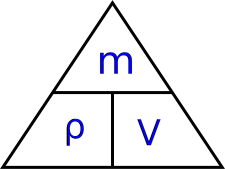
\includegraphics[scale=0.5]{images/pyramide_fraction.png}
\end{figure}

\subsection*{Le \og 1 \fg{} fantôme}

On remarque que
\begin{equation}
\rho = \frac{\rho}{1} \quad \text{donc} \quad \frac{\rho}{1} = \frac{m}{V}.
\nonumber
\end{equation}
On procède comme pour des fractions classiques.

\subsection*{Application numérique}

Remplacer les symboles par des valeurs numériques : si on choisit par exemple $\rho=3$, $m=6$ et $V=2$ on peut réorganiser autant que l'on souhaite l'égalité
\begin{equation}
3=\frac{6}{2}
\nonumber
\end{equation}
tant qu'elle reste vraie.
Il suffit ensuite de repasser aux symboles pour obtenir la bonne écriture littérale.

\section*{Conversions 1D}

Les préfixes permettent d'alléger l'écriture des résultats.

\begin{table}[h]
\center
\begin{tabular}{l|c|c|c|c|c|c|c}
préfixe         & kilo & hecto& déca & ...  & déci & centi& milli\\
abréviation     & k... & h... & da...& ...  & d... & c... & m... \\
facteur         & 1000 & 100  & 10   & 1    & 0{,}1& 0{,}01& 0{,}001 \\
puissance de 10 &$10^3$&$10^2$&$10^1$&$10^0$&$10^{-1}$&$10^{-2}$&$10^{-3}$ 

\end{tabular}
\caption{Quelques préfixes courants.}
\end{table}

\section*{Conversions 3D}

Important pour les volumes !

\begin{didascalie}
Il faut surtout retenir que $\unit{1}{\deci\meter^3}=\unit{1}{\liter}$.
\end{didascalie}



\section*{Puissances de 10}


\end{document}